\documentclass[12pt,a4paper]{article}
\usepackage{amsmath,amssymb,mathrsfs,tikz,times,pifont}
\usepackage[T1]{fontenc}
\usepackage{enumitem}
\newcommand\circitem[1]{%
\tikz[baseline=(char.base)]{
\node[circle,draw=gray, fill=red!55,
minimum size=1.2em,inner sep=0] (char) {#1};}}
\newcommand\boxitem[1]{%
\tikz[baseline=(char.base)]{
\node[fill=cyan,
minimum size=1.2em,inner sep=0] (char) {#1};}}
\setlist[enumerate,1]{label=\protect\circitem{\arabic*}}
\setlist[enumerate,2]{label=\protect\boxitem{\alph*}}
%%%::::::by chnini ameur :::::::%%%
\everymath{\displaystyle}
\usepackage[left=1cm,right=1cm,top=1cm,bottom=1.7cm]{geometry}
\usepackage[colorlinks=true, linkcolor=blue, urlcolor=blue, citecolor=blue]{hyperref}
\usepackage{array,multirow}
\usepackage[most]{tcolorbox}
\usepackage{varwidth}
\usepackage{float} %pour utiliser l'option [H] qui force l'image à apparaître exactement à l'endroit où elle est placée dans le code.
\tcbuselibrary{skins,hooks}
\usetikzlibrary{patterns}
%%%::::::by chnini ameur :::::::%%%
\newtcolorbox{exa}[2][]{enhanced,breakable,before skip=2mm,after skip=5mm,
colback=yellow!20!white,colframe=black!20!blue,boxrule=0.5mm,
attach boxed title to top left ={xshift=0.6cm,yshift*=1mm-\tcboxedtitleheight},
fonttitle=\bfseries,
title={#2},#1,
% varwidth boxed title*=-3cm,
boxed title style={frame code={
\path[fill=tcbcolback!30!black]
([yshift=-1mm,xshift=-1mm]frame.north west)
arc[start angle=0,end angle=180,radius=1mm]
([yshift=-1mm,xshift=1mm]frame.north east)
arc[start angle=180,end angle=0,radius=1mm];
\path[left color=tcbcolback!60!black,right color = tcbcolback!60!black,
middle color = tcbcolback!80!black]
([xshift=-2mm]frame.north west) -- ([xshift=2mm]frame.north east)
[rounded corners=1mm]-- ([xshift=1mm,yshift=-1mm]frame.north east)
-- (frame.south east) -- (frame.south west)
-- ([xshift=-1mm,yshift=-1mm]frame.north west)
[sharp corners]-- cycle;
},interior engine=empty,
},interior style={top color=yellow!5}}
%%%%%%%%%%%%%%%%%%%%%%%

\usepackage{fancyhdr}
\usepackage{eso-pic}         % Pour ajouter des éléments en arrière-plan
% Commande pour ajouter du texte en arrière-plan
\usepackage{tkz-tab}
\AddToShipoutPicture{
    \AtTextCenter{%
        \makebox[0pt]{\rotatebox{80}{\textcolor[gray]{0.7}{\fontsize{5cm}{5cm}\selectfont PGB}}}
    }
}
\usepackage{lastpage}
\fancyhf{}
\pagestyle{fancy}
\renewcommand{\footrulewidth}{1pt}
\renewcommand{\headrulewidth}{0pt}
\renewcommand{\footruleskip}{10pt}
\fancyfoot[R]{
\color{blue}\ding{45}\ \textbf{2025}
}
\fancyfoot[L]{
\color{blue}\ding{45}\ \textbf{Prof:M. BA}
}
\cfoot{\bf
\thepage /
\pageref{LastPage}}
\usetikzlibrary{trees} % Bibliothèque pour les arbres
\newtcolorbox{resultbox}{
    colback=red!30, % Fond rouge clair
    colframe=black, % Bordure noire fine
    sharp corners, % Coins nets
    boxrule=0.5pt, % Contour l\'eger
    boxsep=2pt, % Espacement interne
    left=5pt, right=5pt, top=2pt, bottom=2pt, % Marges internes
}
\begin{document}
\renewcommand{\arraystretch}{1.5}
\renewcommand{\arrayrulewidth}{1.2pt}
\begin{tikzpicture}[overlay,remember picture]
\node[draw=blue,line width=1.2pt,fill=purple,text=blue,inner sep=3mm,rounded corners,pattern=dots]at ([yshift=-2.5cm]current page.north) {\begingroup\setlength{\fboxsep}{0pt}\colorbox{white}{\begin{tabular}{|*1{>{\centering \arraybackslash}p{0.28\textwidth}} |*2{>{\centering \arraybackslash}p{0.2\textwidth}|} *1{>{\centering \arraybackslash}p{0.19\textwidth}|} }
\hline
\multicolumn{3}{|c|}{$\diamond$$\diamond$$\diamond$\ \textbf{Lycée de Dindéfélo}\ $\diamond$$\diamond$$\diamond$ }& \textbf{A.S. : 2024/2025} \\ \hline
\textbf{Matière: Mathématiques}& \textbf{Niveau : T}\textbf{S2} &\textbf{Date: 22/05/2025} & \textbf{Durée : 4 heures} \\ \hline
\multicolumn{4}{|c|}{\parbox[c]{10cm}{\begin{center}
\textbf{{\Large\sffamily Correction Composition Du 2$ ^\text{\bf nd} $ Semestre}}
\end{center}}} \\ \hline
\end{tabular}}\endgroup};
\end{tikzpicture}
\vspace{3cm}

\section*{Exercice 2 \hfill 06 points}

Dans le plan complexe rapporté à un repère orthonormé \( (O ; \vec{u}, \vec{v}) \) d’unité graphique \( 1\,\text{cm} \), on considère les points \( A_0, A_1, A_2 \) d’affixe respective \( z_0 = 5 - 4i \), \( z_1 = -1 - 4i \), \( z_2 = -4 - i \).

Soit \( f \) la fonction qui, à tout point \( M(z) \), associe le point \( M'(z') \), tel que :
\[
z' = \frac{1 - i}{2} z + \frac{-3 + i}{2}
\]

\begin{enumerate}
    \item 
    \begin{enumerate}
        \item Trouver l’affixe \( b \) du point \( B \) invariant par \( f \). \hfill \textbf{(0,5pt)}
    \end{enumerate}

\end{enumerate}

\section*{\underline{PROBLEME} \hfill (10pt)}

\subsection*{PARTIE A}

Soit \( h \) la fonction dérivable sur \( \mathbb{R} \) définie par \( h(x) = 1 + e^{2x - 4} \) et \( K = \left[ 1 ; \frac{5}{4} \right] \).

\begin{enumerate}
    \item
          \begin{enumerate}
              \item[a)] Calcul de \( h'(x) \) :
                  \(
                  h(x) = 1 + e^{2x - 4} \Rightarrow h'(x) =  \left(1 + e^{2x - 4} \right)' = 2e^{2x - 4}
                  \)

                  Comme \( e^{2x - 4} > 0 \) pour tout \( x \in \mathbb{R} \), on a :
                  \(
                  h'(x) > 0 \quad \text{pour tout } x \in \mathbb{R}
                  \)
                  Donc, la fonction \( h \) est **strictement croissante** sur \( \mathbb{R} \). \hfill \textbf{(0,25pt + 0,25pt)}

              \item[b)] Montrons que \( h(K) \subset K \) :

                  Comme \( h \) est croissante et \( K = \left[1 ; \frac{5}{4}\right] \), on a :
                  \[
                      h(K) = \left[ h(1) ; h\left(\frac{5}{4}\right) \right]
                  \]

                  Calculons :
                  \[
                      h(1) = 1 + e^{2(1) - 4} = 1 + e^{-2} \approx 1 + 0{,}1353 = 1{,}1353
                  \]
                  \[
                      h\left(\frac{5}{4}\right) = 1 + e^{2 \cdot \frac{5}{4} - 4} = 1 + e^{-1{,}5} \approx 1 + 0{,}2231 = 1{,}2231
                  \]

                  Donc :
                  \[
                      h(K) = \left[1{,}1353 ; 1{,}2231\right] \subset \left[1 ; \frac{5}{4}\right]
                  \]

                  Ainsi, \( h(K) \subset K \). \hfill \textbf{(0,5pt)}
          \end{enumerate}
    \item
          \begin{enumerate}
              \item[a)] Resoudre \( h(x) = x \)  revient à resoudre \( h(x) - x = 0 \)

                  On définit la fonction \( \phi(x) = h(x) - x = 1 + e^{2x - 4} - x \).

                  \textcolor{red}{\textbf{Existance}}

                  \( \phi \) est continue sur \( K = \left[1 ; \frac{5}{4} \right] \).\\
                  Calculons :
                  \[
                      \phi(1) = 1 + e^{-2} - 1 = e^{-2} > 0 \quad ; \quad \phi\left( \frac{5}{4} \right) = 1 + e^{-1.5} - \frac{5}{4} \approx 1.2231 - 1.25 < 0
                  \]

                  Donc, \( \phi(1) > 0 \) et \( \phi\left( \frac{5}{4} \right) < 0 \), par le théorème des valeurs intermédiaires, il existe un \( \lambda \in \left] 1 ; \frac{5}{4} \right[ \) tel que \( \phi(\lambda) = 0 \), soit \( h(\lambda) = \lambda \).\\

                      \textcolor{red}{\textbf{Unicité}}

                      \[
                          \phi'(x) = h'(x) - 1 = 2e^{2x - 4} - 1
                      \]

                      Supposons que \(\phi'(x)<0\)

                      \(
                      \begin{aligned}
                          \phi'(x) < 0 & \Longleftrightarrow 2e^{2x - 4} - 1 < 0                  \\
                                       & \Longleftrightarrow e^{2x - 4} < \frac{1}{2}             \\
                                       & \Longleftrightarrow 2x - 4 < \ln\left(\frac{1}{2}\right) \\
                                       & \Longleftrightarrow 2x < 4 - \ln(2)                      \\
                                       & \Longleftrightarrow x < 2 - \frac{\ln(2)}{2}             \\
                                       & \Longleftrightarrow x < 1,7
                      \end{aligned}
                      \)

                      Donc si \( x\in ]-\infty ;1,7[ \) alors \(\phi'(x) < 0\)

                  Comme \( K = \left[1 ; \frac{5}{4} \right] \subset ]-\infty ;1,7[ \) donc \( \forall x \in K\, , \phi'(x) < 0\)

                  Donc \( \phi'(x) < 0 \) sur \( K \), donc \( \phi \) est strictement décroissante sur \( K \).\\

                  Or, une fonction continue et strictement monotone sur un intervalle admet **au plus une** racine. Comme on a déjà montré l’existence d’un \( \lambda \), on en déduit que :

                  \[
                      \text{L’équation } h(x) = x \text{ admet une \textbf{unique solution} } \lambda \in K.
                  \] \hfill \textbf{(0,5pt)}

              \item[b)] On a : \( h'(x) = 2e^{2x - 4} \)

                  Encadrons \( x \in K = \left[1 ; \frac{5}{4} \right] \) :

                  \begin{equation*}
                      \begin{aligned}
                          x \in K & \implies 1 \leq x \leq \frac{5}{4}                                       \\
                                  & \implies 2 \leq 2x \leq \frac{5}{2}                                      \\
                                  & \implies -2 \leq 2x - 4 \leq -\frac{3}{2}                                \\
                                  & \implies e^{-2} \leq e^{2x - 4} \leq e^{-1.5}                            \\
                                  & \implies 2e^{-2} \leq 2e^{2x - 4} \leq 2e^{-1.5}                         \\
                                  & \implies 0 \leq 2e^{-2} \leq 2e^{2x - 4} \leq 2e^{-1.5} \leq \frac{1}{2} \\
                                  & \implies 0 \leq 2e^{2x - 4} \leq \frac{1}{2}
                      \end{aligned}
                  \end{equation*}

                  Donc : \( \forall x \in K, \quad 0 < h'(x) < \frac{1}{2} \) \hfill \textbf{(0,25pt)}
              \item[c)] Soit \( x \in K \), et \( \lambda \in K \) l’unique solution de \( h(\lambda) = \lambda \).

                  D’après l’inégalité des accroissements finis (ou le théorème de la moyenne) appliquée à \( h \) sur \( K \), il existe \( c \in [x ; \lambda] \subset K \) tel que :
                  \[
                      h(x) - h(\lambda) = h(x) - \lambda = h'(c)(x - \lambda)
                  \]
                  Donc :
                  \[
                      |h(x) - \lambda| = |h'(c)| \times |x - \lambda| \leq \frac{1}{2} |x - \lambda|
                  \]
                  \hfill \textbf{(0,25pt)}
          \end{enumerate}

    \item[3.a)] Montrons par récurrence que \( \forall n \in \mathbb{N},\ W_n \in K \).

        \textcolor{red}{\textbf{Initialisation :}}\\
        On a \( W_0 = 1 \in K = \left[1 ; \frac{5}{4} \right] \). L’assertion est vraie au rang \( n = 0 \).

        \textcolor{red}{\textbf{Hérédité :}}\\
        Supposons que pour un entier \( n \in \mathbb{N} \), on ait \( W_n \in K \).\\
        Alors par définition :
        \[
            W_{n+1} = h(W_n)
        \]
        Or à la question 1.b), on a démontré que \( h(K) \subset K \).\\
        Donc comme \( W_n \in K \), on a \( W_{n+1} \in h(K) \subset K \).\\

        \textcolor{red}{\textbf{Conclusion :}}\\
        Par le principe de récurrence, on a :
        \[
            \forall n \in \mathbb{N},\quad W_n \in K
        \]
        \hfill \textbf{(0,5pt)}

    \item[b)] On veut montrer que :
        \[
            |W_{n+1} - \lambda| \leq \frac{1}{2}|W_n - \lambda| \quad \text{et} \quad |W_n - \lambda| \leq \left( \frac{1}{2} \right)^n, \quad \forall n \in \mathbb{N}
        \]

        \textcolor{red}{\textbf{1) Inégalité de récurrence :}}\\
        On sait que \( W_{n+1} = h(W_n) \) et que \( \lambda \) est l’unique solution de \( h(\lambda) = \lambda \).\\
        D’après la question 2.c), on a pour tout \( x \in K \) :
        \[
            |h(x) - \lambda| \leq \frac{1}{2} |x - \lambda|
        \]
        Or, à la question 3.a), on a montré que \( \forall n, \ W_n \in K \). Donc :
        \[
            |W_{n+1} - \lambda| = |h(W_n) - \lambda| \leq \frac{1}{2} |W_n - \lambda|
        \]

        \textcolor{red}{\textbf{2) Majoration par \( \left( \frac{1}{2} \right)^n \) par récurrence :}}\\

    \item[3.b)] On a \( W_{n+1} = h(W_n) \) et \( h(\lambda) = \lambda \).\\
        D’après la question 2.c), pour tout \( x \in K \), on a :
        \[
            |h(x) - \lambda| \leq \frac{1}{2} |x - \lambda|
        \]
        Or, à la question 3.a), on a montré que \( W_n \in K \) pour tout \( n \in \mathbb{N} \), donc on peut appliquer cette inégalité à chaque itération :

        \begin{equation*}
            \begin{aligned}
                |W_{1} - \lambda| & \leq \frac{1}{2} |W_0 - \lambda|     \\
                |W_{2} - \lambda| & \leq \frac{1}{2} |W_1 - \lambda|     \\
                |W_{3} - \lambda| & \leq \frac{1}{2} |W_2 - \lambda|     \\
                                  & \ \vdots                             \\
                |W_k - \lambda|   & \leq \frac{1}{2} |W_{k-1} - \lambda|
            \end{aligned}
        \end{equation*}

        En multipliant ces inégalités **membre à membre**, on obtient :

        \begin{equation*}
            |W_k - \lambda| \leq \left( \frac{1}{2} \right)^k |W_0 - \lambda|
        \end{equation*}

        \[
            \forall k \in \mathbb{N},\quad |W_k - \lambda| \leq \left( \frac{1}{2} \right)^k
        \]

        \hfill \textbf{(0,5pt + 0,25pt)}
    \item[c)] D’après la question précédente, on a :
        \[
            |W_n - \lambda| \leq \left( \frac{1}{2} \right)^n
        \]

        Or \( \left( \frac{1}{2} \right)^n \to 0 \) quand \( n \to +\infty \), donc :
        \[
            |W_n - \lambda| \to 0
            \quad \text{ce qui équivaut à} \quad
            W_n \to \lambda
            \quad \text{quand } n \to +\infty
        \]

        Ainsi, la suite \( (W_n) \) **converge vers le réel \( \lambda \)**, qui est l’unique solution de l’équation \( h(x) = x \) dans l’intervalle \( K \). \hfill \textbf{(0,25pt)}

\end{enumerate}

\subsection*{PARTIE B}

Soit \( f \) la fonction définie par :
\[
    f(x) =
    \begin{cases}
        \ln\left( \left| \dfrac{x - 1}{x + 1} \right| \right) & \text{si } x \in [0 ; +\infty[ \\
        \displaystyle x-\frac{e^x - 1}{e^x + 1}               & \text{si } x \in ]-\infty ; 0[
    \end{cases}
\]

\begin{enumerate}
    \item Déterminons le domaine de définition \( D_f \) de \( f \).\\

          \textcolor{red}{\textbf{Sur } \( [0 ; +\infty[ \)} : on considère l’expression
          \[
              f(x) = \ln\left( \left| \frac{x - 1}{x + 1} \right| \right)
          \]
          Cette expression est définie si :
          \begin{itemize}
              \item \( x + 1 \neq 0 \Rightarrow x \neq -1 \) (toujours vrai car \( x \geq 0 \))
              \item \( \left| \frac{x - 1}{x + 1} \right| > 0 \Rightarrow \frac{x - 1}{x + 1} \neq 0 \Rightarrow x \neq 1 \)
          \end{itemize}
          Donc sur \( [0 ; +\infty[ \), la fonction est définie sauf en \( x = 1 \).\\

          \textcolor{red}{\textbf{Sur } \( ]-\infty ; 0[ \)} : on considère
                  \[
                      f(x) = x-\frac{e^x - 1}{e^x + 1}
                  \]
                  Cette expression est définie pour tout \( x \in \mathbb{R} \), car le dénominateur \( e^x + 1 > 0 \) pour tout \( x \).\\

                  Donc la fonction \( f \) est définie sur :
                  \[
                  D_f = ]-\infty ; 1[ \cup ]1 ; +\infty[
          \]
          \hfill \textbf{(0,5pt)}

    \item[2.] Étudions la continuité de \( f \) en 0.\\

        La fonction \( f \) est définie par morceaux :

        \[
            f(x) =
            \begin{cases}
                \ln\left( \left| \frac{x - 1}{x + 1} \right| \right) & \text{si } x \in [0 ; +\infty[ \\
                x-\frac{e^x - 1}{e^x + 1}                            & \text{si } x \in ]-\infty ; 0[
            \end{cases}
        \]

        A-t-on \( \displaystyle \lim_{x \to 0^-} f(x) = \lim_{x \to 0^+} f(x) = f(0) \) ?

        \textcolor{red}{\textbf{Limite à gauche (vers 0\(^-\)) :}}\\
        Pour \( x < 0 \),

        \(
        \begin{aligned}
            \lim\limits_{x\to 0^{-} }f(x) & = \lim\limits_{x\to 0^{-} }x-\frac{e^x - 1}{e^x + 1} \\
                                          & =0- \frac{1 - 1}{1 + 1}                              \\
                                          & = 0
        \end{aligned}
        \)

        \begin{resultbox}
            \[
                \mathbf{\lim\limits_{x\to 0^{-} }f(x)=0}
            \]
        \end{resultbox}

        \textcolor{red}{\textbf{Limite à droite (vers 0\(^+\)) :}}\\
        Pour \( x > 0 \),

        \(
        \begin{aligned}
            \lim\limits_{x\to 0^{+} }f(x) & =\ln\left( \left| \frac{x - 1}{x + 1} \right| \right) \\
                                          & =\ln\left( \left| \frac{-1}{1} \right| \right)        \\
                                          & =\ln(1)                                               \\
                                          & = 0                                                   \\
        \end{aligned}
        \)

        \begin{resultbox}
            \[
                \mathbf{\lim\limits_{x\to 0^{+} }f(x)=0}
            \]
        \end{resultbox}

        \textcolor{red}{\textbf{Conclusion :}}\\
        La limite de \( f(x) \) en 0 existe et vaut 0.\\
        De plus, \( f(0) = \ln\left( \left| \frac{0 - 1}{0 + 1} \right| \right) = \ln(1) = 0 \)

        \begin{resultbox}
            \[
                \mathbf{Donc :  \lim_{x \to 0^-} f(x) = \lim_{x \to 0^+} f(x) = f(0) \Rightarrow f \text{ est continue en } 0 }
            \]
        \end{resultbox}
    \item
          \begin{enumerate}
              \item Soit \( x \in ]0 ; 1[ \).\\

                    On a : \( x < 1 \), donc \( x - 1 < 0 \), donc : \( |x - 1| = -(x - 1) = 1 - x \)

                    De plus, dans ce cas \( x > 0 \), donc \( f(x) = \ln\left( \left| \frac{x - 1}{x + 1} \right| \right) \).\\
                    On remplace \( |x - 1| \) par \( 1 - x \), et on obtient : \( f(x) = \ln\left( \frac{1 - x}{x + 1} \right) \)

                    Or, on sait que : \( \ln\left( \frac{1 - x}{1 + x} \right) = \ln(1 - x) - \ln(1 + x) \)

                    Donc : \(     f(x) = \ln(1 - x) - \ln(1 + x) \Rightarrow \frac{f(x)}{x} = \frac{\ln(1 - x)}{x} - \frac{\ln(1 + x)}{x} \) \hfill \textbf{(0,5pt)}

              \item Étudions la dérivabilité de \( f \) en 0.

                    On cherche la limite du taux d’accroissement :\(\lim\limits_{x \to 0} \frac{f(x) - f(0)}{x}
                    \quad \text{avec } f(0) = 0 \ \text{(voir question 2)}\)

                    %Il s'agit donc d'étudier : \( \lim\limits_{x \to 0} \frac{f(x)}{x} \)

                    \textcolor{red}{\textbf{À gauche (} \( x \to 0^- \) \textbf{) :}}\\
                    \(
                    \begin{aligned}
                        \lim\limits_{x \to 0^-} \frac{f(x)-f(0)}{x-0} & = \lim\limits_{x \to 0^-}\frac{f(x)}{x}                                \\
                                                                      & = \lim\limits_{x \to 0^-}\frac{x-\dfrac{e^x - 1}{e^x + 1}}{x}          \\
                                                                      & = \lim\limits_{x \to 0^-}1- \frac{e^x - 1}{x} \times \frac{1}{e^x + 1} \\
                                                                      & =1 - 1 \times\frac{1}{2}                                               \\
                                                                      & =\frac{1}{2}
                    \end{aligned}
                    \)

                    \begin{resultbox}
                        \[
                            \mathbf{\lim\limits_{x \to 0^-} \frac{f(x)-f(0)}{x-0}=\frac{1}{2}}
                        \]
                    \end{resultbox}

                    \textcolor{red}{\textbf{À droite (} \( x \to 0^+ \) \textbf{) :}}\\

                    \(
                    \begin{aligned}
                        \lim\limits_{x \to 0^+} \frac{f(x)-f(0)}{x-0} & = \lim\limits_{x \to 0^+} \frac{f(x)}{x}                             \\
                                                                      & = \lim\limits_{x \to 0^+}\frac{\ln(1 - x)}{x} - \frac{\ln(1 + x)}{x} \\
                                                                      & =-1-1                                                                \\
                                                                      & =-2
                    \end{aligned}
                    \)

                    \begin{resultbox}
                        \[
                            \mathbf{\lim\limits_{x \to 0^+} \frac{f(x)-f(0)}{x-0}=-2}
                        \]
                    \end{resultbox}

                    \textcolor{red}{\textbf{Conclusion :}}\\

                    \begin{resultbox}
                        \[
                            \mathbf{\lim\limits_{x \to 0^+} \frac{f(x)-f(0)}{x-0}=-2 \text{ et } \lim\limits_{x \to 0^-} \frac{f(x)-f(0)}{x-0}=\frac{1}{2}}
                        \]
                    \end{resultbox}

                    Donc la fonction \( f \) **n’est pas dérivable** en 0. \hfill \textbf{(0,5pt)}

              \item 
                    \textcolor{red}{\textbf{À gauche de 0 :}}\\
                    La pente de la demi-tangente est \( \frac{1}{2} \), donc l'équation de la tangente gauche est :
                    \[
                        y = \frac{1}{2}x
                    \]

                    \textcolor{red}{\textbf{À droite de 0 :}}\\
                    La pente de la demi-tangente est \( -2 \), donc l'équation de la tangente droite est :
                    \[
                        y = -2x
                    \]

                    \begin{resultbox}
                        \[
                            y = \frac{1}{2}x \quad \text{et} \quad y = -2x \quad\quad \textbf{(0,5pt)}
                        \]
                    \end{resultbox}

          \end{enumerate}

    \item Montrons que \( \forall x \in ]-\infty ; 0[ \), \( f(x) = x - \frac{e^x - 1}{e^x + 1} = x + 1 - \frac{2e^x}{e^x + 1} \)

          \textcolor{red}{\textbf{Démonstration :}}

          Partons du membre de droite :
          \(
            \begin{aligned}
                x + 1 - \frac{2e^x}{e^x + 1}&= \frac{(x + 1)(e^x + 1) - 2e^x}{e^x + 1}\\
                                            &= \frac{x e^x + x + e^x + 1
                                            - 2e^x}{e^x + 1}\\
                                            &=\frac{x e^x + x - e^x + 1}{e^x + 1}\\
                                            &=\frac{x(e^x + 1)}{e^x + 1}+\frac{- e^x + 1}{e^x + 1}\\
                                            &=x+\frac{- e^x + 1}{e^x + 1}\\
                                            &=x-\frac{ e^x - 1}{e^x + 1} \textbf{ CQFD}\\
            \end{aligned}
         \)

         \hfill \textbf{(0,25pt)}

         \item Calculons les limites de \( f \) aux bornes des intervalles de son domaine de définition. \hfill \textbf{(0,5pt)}

\textcolor{red}{\textbf{À gauche de 1 :}} \( x \to 1^- \)

Sur \( [0 ; 1[ \), on a : \( f(x) = \ln\left( \left| \frac{x - 1}{x + 1} \right| \right) = \ln\left( \frac{1 - x}{x + 1} \right) \)

\(
\begin{aligned}
    \lim\limits_{x \to 1^-} f(x) &= \lim\limits_{x \to 1^-} \ln\left( \frac{1 - x}{x + 1} \right)\\
                                &= \ln(0^+)\\
                                & = -\infty
\end{aligned}
\)

\begin{resultbox}
\[
\boxed{\lim_{x \to 1^-} f(x) = -\infty}
\]
\end{resultbox}

\textcolor{red}{\textbf{À droite de 1 :}} \( x \to 1^+ \)

Sur \( ]1 ; +\infty[ \), même expression : \( f(x) = \ln\left( \left| \frac{x - 1}{x + 1} \right| \right) \)

\(
\begin{aligned}
    \lim\limits_{x \to 1^+} f(x) &= \ln\left( \frac{x - 1}{x + 1} \right)\\ 
                                 &= \ln(0^+)\\
                                 &= -\infty
\end{aligned}
\)

\begin{resultbox}
\[
\boxed{\lim_{x \to 1^+} f(x) = -\infty}
\]
\end{resultbox}

\textcolor{red}{\textbf{À gauche de 0 :}} \( x \to -\infty \)

Sur \( ]-\infty ; 0[ \), on a \( f(x) = x - \frac{e^x - 1}{e^x + 1} \).\\

\(
\begin{aligned}
    \lim\limits_{x\to -\infty}f(x)&=\lim\limits_{x\to -\infty}x-\frac{e^x - 1}{e^x + 1}\\
                                  &= -\infty - \frac{-1}{1}\\
                                  &=-\infty
\end{aligned}
\)

\begin{resultbox}
\[
\boxed{\lim_{x \to -\infty} f(x) = -\infty}
\]
\end{resultbox}

\textcolor{red}{\textbf{À droite de 0 :}} \( x \to +\infty \)

Sur \( ]1 ; +\infty[ \), \( f(x) = \ln\left( \left| \frac{x - 1}{x + 1} \right| \right) \).\\

\(
\begin{aligned}
    \lim\limits_{x\to +\infty}f(x)&=\lim\limits_{x\to +\infty}\ln\left( \left| \frac{x - 1}{x + 1} \right| \right)\\
                                  &= \ln(1)\\
                                  &=0
\end{aligned}
\)

\begin{resultbox}
\[
\boxed{\lim_{x \to +\infty} f(x) = 0}
\]
\end{resultbox}

\item En déduire les équations des asymptotes à la courbe \( \mathscr{C}_f \) de \( f \). \hfill \textbf{(0,25pt)}

\textcolor{red}{\textbf{Asymptote verticale :}}

D’après la question précédente, on a :
\[
\lim_{x \to 1^-} f(x) = \lim_{x \to 1^+} f(x) = -\infty
\]

Donc la droite \( x = 1 \) est une \textbf{asymptote verticale} à la courbe \( \mathscr{C}_f \).

\vspace{0.5em}
\textcolor{red}{\textbf{Asymptote horizontale :}}

On a également :
\[
\lim_{x \to +\infty} f(x) = 0
\]

Donc la droite \( y = 0 \) est une \textbf{asymptote horizontale} à droite de la courbe \( \mathscr{C}_f \).

\begin{resultbox}
\[
\boxed{
\text{Asymptotes de } \mathscr{C}_f :
\quad x = 1 \quad \text{et} \quad y = 0
}
\]
\end{resultbox}

\item Calculer \( f'(x) \) pour tout \( x \in \mathbb{R} \setminus \{0 ; 1\} \). \hfill \textbf{(0,5pt)}

\textcolor{red}{\textbf{Sur } \( ]0 ; 1[ \cup ]1 ; +\infty[ \)} :

Pour \( x > 0 \), on a :
\[
f(x) = \ln\left( \left| \frac{x - 1}{x + 1} \right| \right) = \ln\left( \frac{x - 1}{x + 1} \right) \quad \text{car } \frac{x - 1}{x + 1} > 0
\]

\[
f'(x) = \frac{1}{x+1} - \frac{1}{x-1}\implies  f'(x) =\frac{2}{(x + 1)(x - 1)}
\]

\textcolor{red}{\textbf{Sur } \( ]-\infty ; 0[ \)} :

Pour \( x < 0 \), on a :
\[
f(x) = x - \frac{e^x - 1}{e^x + 1} \text{ou encore} f(x) = x+1 - \frac{2e^x}{e^x + 1}
\]

\[
f'(x)=1 - \frac{2e^x (e^x + 1) - (e^x - 1)(e^x)}{(e^x + 1)^2}
=1- \frac{e^x(e^x + 1 - e^x + 1)}{(e^x + 1)^2}
=1- \frac{2e^x}{(e^x + 1)^2}
\]

Donc :
\[
f'(x) = 1 - \frac{2e^x}{(e^x + 1)^2}
\]

\begin{resultbox}
\[
f'(x) =
\begin{cases}
\displaystyle \frac{2}{(x + 1)(x - 1)} & \text{si } x \in ]0 ; 1[ \cup ]1 ; +\infty[ \\
\\
\displaystyle 1 - \frac{2e^x}{(e^x + 1)^2} & \text{si } x \in ]-\infty ; 0[
\end{cases}
\]
\end{resultbox}

\item Étudier les variations de \( f \). \hfill \textbf{(0,5pt)}

On rappelle que le domaine de définition de \( f \) est :
\[
D_f = ]-\infty ; 1[ \cup ]1 ; +\infty[
\]

\textcolor{red}{\textbf{Sur } \( ]-\infty ; 0[ \)} :

On a montré précédemment :

\(
\begin{aligned}
    f'(x) &= 1 - \frac{2e^x}{(e^x + 1)^2}\\
          &=\frac{(e^x + 1)^2-2e^x}{(e^x + 1)^2}\\
          &=\frac{e^{2x}+2e^x+1-2e^{x}}{(e^x + 1)^2}\\
          &=\frac{e^{2x}+1}{(e^x + 1)^2}>0
\end{aligned}
\)

\[
f'(x) > 0 \text{ sur } ]-\infty ; 0[
\Rightarrow f \text{ est strictement croissante sur } ]-\infty ; 0[
\]

\vspace{1em}

\textcolor{red}{\textbf{Sur } \( ]0 ; 1[ \cup ]1 ; +\infty[ \)} :

On a :
\[
f'(x) = \frac{2}{(x + 1)(x - 1)}
\]

Le signe de \( f'(x) \) dépend du signe de \( (x + 1)(x - 1) \).

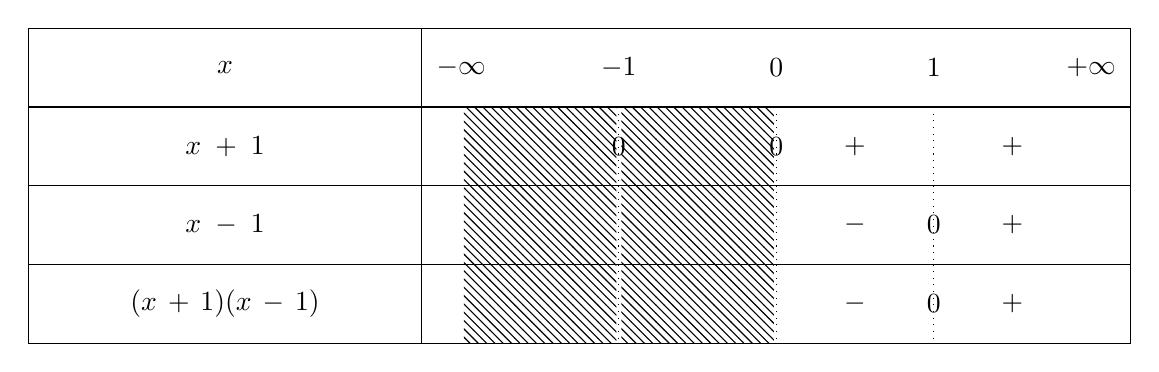
\begin{tikzpicture}
    \tkzTabInit[lgt=5, espcl=2]
        {$x$ / 1 , $x+1$ / 1 , $x-1$ / 1 , $(x + 1)(x - 1)$ / 1}
        {$-\infty$, $-1$, $0$ , $1$, $+\infty$}
    \tkzTabLine{ , h , z , h , z , + , t, + }
    \tkzTabLine{ , h , t , h , t , - , z, + }
    \tkzTabLine{ , h , t , h , t , - , z, + }
\end{tikzpicture}

\begin{itemize}
    \item Sur \( ]0 ; 1[ \), on a \( (x + 1)(x - 1) < 0 \)  
          donc \( f'(x) < 0 \) : \( f \) est décroissante sur \( ]0 ; 1[ \)

    \item Sur \( ]1 ; +\infty[ \), \( (x + 1)(x - 1) > 0 \)  
          donc \( f'(x) > 0 \) : \( f \) est croissante sur \( ]1 ; +\infty[ \)
\end{itemize}

\vspace{1em}

    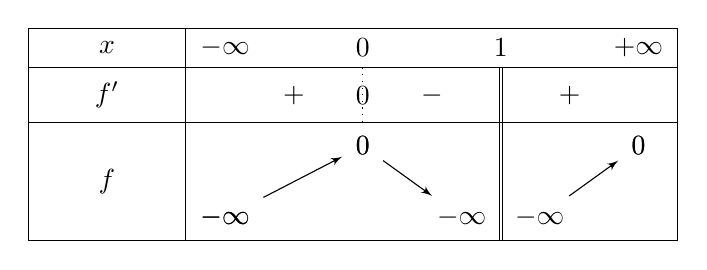
\begin{tikzpicture}[node style/.style={fill opacity=0,text opacity=1}]
        \tkzTabInit[espcl=1.75]{$x$/.5,$f'$/.7,$f$/1.5}{$-\infty$,$0$,$1$,$+\infty$}
        \tkzTabLine{,+,z,-,d,+,}
        \tkzTabVar{-/$-\infty$,+/$0$,-D-/$-\infty$/$-\infty$,+/$0$}
    \end{tikzpicture}

\begin{center}
        \begin{figure}[H]% Forcer l'image à cet endroit
         \centering
         \includegraphics[width=0.8\textwidth]{diopLeParresseux.png}
        \end{figure}
    \end{center}
        \href{https://www.geogebra.org/classic/efgm6ucx}{Clique ici pour voir la figure sur géogébra}

\end{enumerate}

\subsection*{PARTIE C}

Soit \( g \) la restriction de la fonction \( f \) à l’intervalle \( I = ]1 ; +\infty[ \).

\begin{enumerate}
    \item Montrons que \( g \) réalise une bijection de \( I \) vers un intervalle \( J \).

    On a vu que sur \( ]1 ; +\infty[ \), la fonction \( f \) est définie et strictement croissante.\\
    Or une fonction continue et strictement monotone est bijective de son domaine d’étude sur son image.

    \[
    \text{Donc, } g : I \to J \text{ est une bijection.}
    \]

    \[
    J = ]-\infty ; 0[
    \]

    \hfill \textbf{(0,5pt)}

    \item Soit \( y \in J = ]-\infty ; 0[ \). On cherche l'expression de \( g^{-1}(y) \).

    Par définition :
    \[
    y = g(x) = \ln\left( \frac{x - 1}{x + 1} \right) \quad \text{avec } x \in ]1 ; +\infty[
    \]

    Posons \( y = \ln\left( \frac{x - 1}{x + 1} \right) \). Exponentions :
    \[
    e^y = \frac{x - 1}{x + 1}
    \]

    On résout cette équation pour \( x \) :
    \[
    e^y(x + 1) = x - 1 \quad \Rightarrow \quad e^y x + e^y = x - 1
    \]
    \[
    e^y x - x = -1 - e^y \quad \Rightarrow \quad x(e^y - 1) = -1 - e^y
    \]
    \[
    x = \frac{-1 - e^y}{e^y - 1} = \frac{-(1 + e^y)}{e^y - 1} = 1 - \frac{2e^y}{e^y - 1}
    \]

    Donc :
    \[
    g^{-1}(y) = 1 - \frac{2e^y}{e^y - 1}
    \quad \text{soit} \quad
    g^{-1}(x) = 1 - \frac{2e^x}{e^x - 1}
    \]

    \hfill \textbf{(0,25pt)}

    \item Pour tracer la courbe \( \mathcal{C}_{g^{-1}} \), on peut exploiter la symétrie par rapport à la droite \( y = x \), puisque \( g^{-1} \) est la bijection réciproque de \( g \).\\

    On pourra donc obtenir \( \mathcal{C}_{g^{-1}} \) en prenant les points symétriques de ceux de \( \mathcal{C}_g \) par rapport à la droite \( y = x \).\\

    Elle est définie sur \( J = ]-\infty ; 0[ \) et a pour équation :

    \[
    \mathcal{C}_{g^{-1}} : \quad y = g^{-1}(x) = 1 - \frac{2e^x}{e^x - 1}
    \]

    \hfill \textbf{(0,5pt)}
\end{enumerate}

\begin{center}
        \begin{figure}[H]% Forcer l'image à cet endroit
         \centering
         \includegraphics[width=0.8\textwidth]{diopLeParresseuxReciproque.png}
        \end{figure}
    \end{center}
        \href{https://www.geogebra.org/classic/efgm6ucx}{Clique ici pour voir la figure sur géogébra}
\end{document}
